\chapter{Experimentos e Resultados}
\label{ch:07}

O enfoque deste capítulo será em analisar os resultados obtidos pelos experimentos com o modelo encoder-decoder.

falar de type e token

falar que eu tirei o r dos infinitivos pq era redundante

\begin{itemize}
    \item explicar que nessa seção vou analisar os resultados obtidos
    \item introduzir que a acurácia nao foi muito boa e que apesar disso tento entender os resultados dos modelos
    \item falar sobre a dificuldade de interpretação dos resultados de modelos de redes neurais
    \item falar sobre os poucos dados disponíveis%(https://medium.com/scribd-data-science-engineering/experiments-with-seq2seq-data-dependency-62184993f555)
\end{itemize}

\section{Treinamento}

\begin{itemize}
    \item Explicar o que são épocas
    \item explicar o que é batch size
    \item explicar hiperparâmetros
\end{itemize}
\subsection{300 epochs}
\begin{figure}[H]
  \centering
  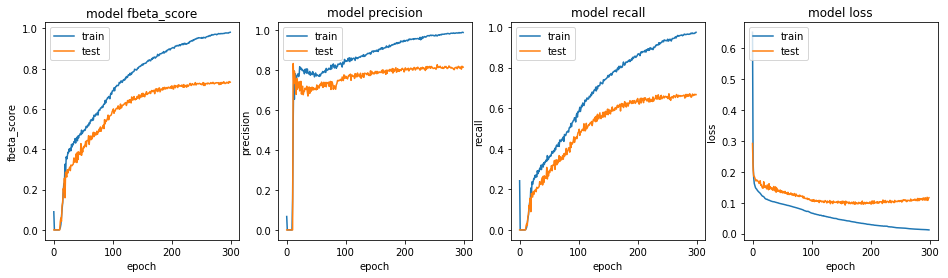
\includegraphics[width=1.0\linewidth]{img/300_fbeta.png}
  \caption{Resultados 300 epocas}
  \label{fig:training}
\end{figure}

Explicar as metricas em analise:
\begin{itemize}
    \item o que representa o f score
    \item o que representa a precision
    \item recall
    \item erro
    \item explicar pq as metricas parecem muito boas
\end{itemize}
\subsection{2000 epochs}


\begin{figure}[H]
  \centering
  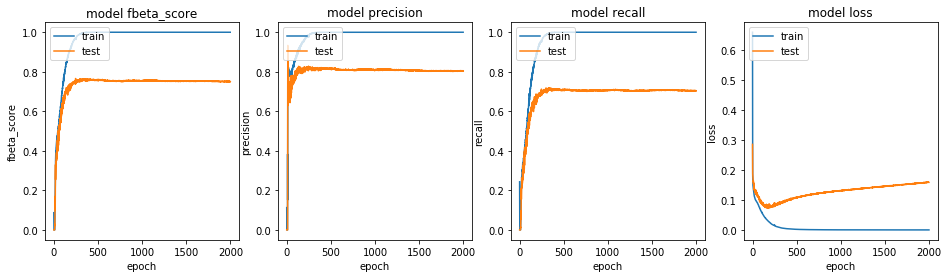
\includegraphics[width=1.0\linewidth]{img/2000_precision.png}
  \caption{Resultados 2000 Epocas}
  \label{fig:encdec}
\end{figure}

Mostrar aonde começa o overfit e discutir que 300 epocas era o suficiente

\section{Análise K-Fold}

Como o tamanho do corpus disponível é restrito, não é interessante realizar um único experimento com uma única segmentação entre treino e teste, pois haveriam verbos em que o modelo nunca seria testado e outros que nunca seriam utilizados no treinamento. Dessa forma a acurácia do modelo poderia variar bastante dependendo dos verbos sorteados para cada um desses grupos. Assim, uma técnina de validação cruzada chamada \textit{K-Fold} foi escolhida para o estudo dos resultados. A análise K-Fold permite que o modelo seja avaliado em todos os verbos do corpus. A técnica consiste, primeiramente, na formação de K subconjuntos de verbos mutuamente exclusivos de tamanhos similares (idênticos caso a divisão por K seja exata). Em seguida, um desses subconjuntos é escolhido como o conjunto de teste enquanto que os K-1 restantes são utilizados como treino. O tamanho de K é definido a partir da escolha de proporção em que se deseja realizar a segmentação entre treino e teste, ou seja, para sempre manter a proporção de testes em 20\% de modo que estes verbos sejam sempre diferentes, o corpus precisa ser segmentado em 5 subconjuntos distintos. O desenho \ref{fig:kfold} ilustra o algoritmo. 

\definecolor{blue}{RGB}{159, 192, 176}
\definecolor{green}{RGB}{160, 227, 127}
\definecolor{orange}{RGB}{243, 188, 125}
\definecolor{red}{RGB}{253, 123, 84}
\definecolor{nephritis}{RGB}{39, 174, 96}
\definecolor{emerald}{RGB}{46, 204, 113}
\definecolor{turquoise}{RGB}{39, 174, 96}
\definecolor{green-sea}{RGB}{22, 160, 133}
\definecolor{purple}{RGB}{181, 124, 215}
% Tikzstyles for Computation Graphs

% nodes
\tikzstyle{noop} = [circle, draw=none, fill=red, minimum size = 10pt]
\tikzstyle{op} = [circle, draw=red, line width=1.5pt, fill=red!70, text=black, text centered, font=\bf \normalsize, minimum size = 25pt]

\tikzstyle{opintense} = [circle, draw=red, line width=1.5pt, fill=red!150, text=black, text centered, font=\bf \normalsize, minimum size = 25pt]


%new style
\tikzstyle{gp} = [circle, draw=red, line width=4pt, text=black, text centered, font=\bf \normalsize, minimum size = 4.cm]

\tikzstyle{box} = [rectangle, draw=red, line width=1.5pt, fill=red!70, text=black, align=center, font=\bf \normalsize, minimum size = 45pt]

\tikzstyle{box2} = [rectangle, draw=black, line width=0.9pt, text=black, align=center, font=\bf \normalsize, minimum size = 20pt]

\tikzstyle{box3} = [rectangle, draw=black, line width=0.9pt, fill=black, text=black, align=center, font=\bf \normalsize, minimum size = 20pt]

\tikzstyle{state} = [circle, draw=blue, line width=1.5pt, fill=blue!70, text=black, text centered, font=\bf \normalsize, minimum size = 25pt]

\tikzstyle{output} = [circle, draw=purple, line width=1.5pt, fill=purple!70, text=black, text centered, font=\bf \normalsize, minimum size = 25pt]


\tikzstyle{gradient} = [circle, draw=nephritis, line width=1.5pt, fill=nephritis!60, text=black, text centered, font=\bf \normalsize, minimum size = 25pt]
\tikzstyle{textonly} = [draw=none, fill=none, text centered, font=\bf \normalsize]
\tikzstyle{boxtextonly} = [draw=none, fill=none, align=center, font=\bf \normalsize]

\tikzstyle{normal} = [circle, draw=black, line width=1.0pt, fill=none, text=black, text centered, font=\bf \normalsize, minimum size = 20pt]


% edges
\tikzstyle{tedge}  = [draw, thick, >=latex, ->]
\tikzstyle{tedge_dashed}  = [draw, thick, >=latex, ->, dashed]
\tikzstyle{nedge}  = [draw, thick, >=latex]
\tikzstyle{nedge_dashed}  = [draw, thick, >=latex, dashed]


% namedscope
\tikzstyle{namedscope} = [circle, draw=orange, line width=1.5pt, fill=orange!60, align=center, inner sep=0pt]
\begin{figure}[ht!]
\centering

\scalebox{1.0}{
\begin{tikzpicture}[H]

%first
\node[box3] (box1) {};
\node[box2, right=0pt of box1] (box2) {};
\node[box2, right=0pt of box2] (box3) {};
\node[box2, right=0pt of box3] (box4) {};
\node[box2, right=0pt of box4] (box5);

%second
\node[box2, below=15pt of box1] (box6) {};
\node[box3, right=0pt of box6] (box7) {};
\node[box2, right=0pt of box7] (box8) {};
\node[box2, right=0pt of box8] (box9) {};
\node[box2, right=0pt of box9] (box10);

%third
\node[box2, below=15pt of box6] (box11) {};
\node[box2, right=0pt of box11] (box12) {};
\node[box3, right=0pt of box12] (box13) {};
\node[box2, right=0pt of box13] (box14) {};
\node[box2, right=0pt of box14] (box15);

%fourth
\node[box2, below=15pt of box11] (box16) {};
\node[box2, right=0pt of box16] (box17) {};
\node[box2, right=0pt of box17] (box18) {};
\node[box3, right=0pt of box18] (box19) {};
\node[box2, right=0pt of box19] (box20);

%fifth
\node[box2, below=15pt of box16] (box21) {};
\node[box2, right=0pt of box21] (box22) {};
\node[box2, right=0pt of box22] (box23) {};
\node[box2, right=0pt of box23] (box24) {};
\node[box3, right=0pt of box24] (box25);

%legenda
\node[box2, right=35pt of box10] (box26) {};
\node[textonly, right=5pt of box26] (box27) {Treino};
\node[box3, below=10pt of box26] (box28) {};
\node[textonly, right=5pt of box28] (box29) {Teste};



\end{tikzpicture}
}\caption{Técnica de segmentação do Corpus via K-Fold} 
\label{fig:kfold}
\end{figure}

Além disso, há ainda a vantagem do elemento de estratificação, ou seja, a possibilidade de que em cada um doss treinamentos, as proporções das classes de verbos se mantenham no treinamento. Isso significa que, por exemplo, a classe de irregularidades 12 (testar -> tEstu) que possui 20 verbos, terá sempre 16 verbos verbos no treinamento e 4 no teste. Assim, após os 5 treinamentos diferentes, todos os verbos da classe foram testados e há a certeza de que haviam verbos dessa classe no treinamento. 

Ainda, como há um fator de aleatoriedade devido às inicializações dos pesos e também como os itens de treino e teste são sorteados pelo algoritmo no momento da segmentação do K-Fold, os resultados da rede podem variar. Para uma melhor compreensão de como ocorre essa variação para cada classe, foram realizadas 30 análises K-Fold. Dentre esses experimentos, a acurácia mais alta obtida foi de 17\% (73 verbos). As análises a seguir foram feitas no intuito de se entender melhor as situações de maior dificuldade do modelo.

\subsection{A relação entre acurácia e a proporção da classe no corpus}
Um fator que pode influenciar no resultado é o tamanho do corpus e o desbalanceamento das classes. O modelo encoder-decoder é normalmente executado com uma variedade de dezenas de milhares de exemplos. Portanto, cabe verificar se há alguma relação entre a proporção da classe no corpus e a acurácia. Na Fig.\ref{fig:kfoldprop} é possível observar que as acurácias de algumas das classes de verbos seguem uma certa tendência linear de acordo com as suas respectivas proporções no corpus, enquanto que há um outro grupo de classes que apresenta acurácia mais baixa independentemente da proporção.

\begin{figure}[H]
  \centering
  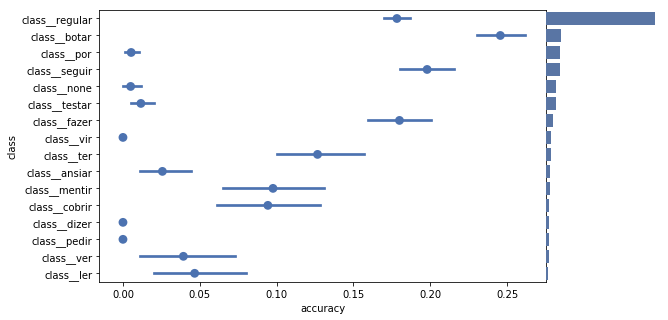
\includegraphics[width=0.8\linewidth]{img/accuracy_kfold_1.png}
  \caption{Acurácia Ordenada pela Proporção das Classes}
  \label{fig:kfoldprop}
\end{figure}

O experimento com acurácia mais alta será utilizado como referência para a análise de erros.

Ao analisar os erros ocorridos na classe do verbo "Pôr" (vide apêndice), verifica-se que praticamente um terço (8/26) dos erros foram erros de "regularização", ou seja, o modelo se confundiu com a classe mais presente (de verbos regulares). 

Em seguida, a próxima classe com acurácia baixa fora da tendência é a classe de verbos sem agrupamento. Esse resultado era totalmente esperado pois não havia outros verbos no corpus para que o modelo conseguisse detectar possíveis padrões para fazer predições corretas. 

A classe do verbo "testar" apresentou muitas predições incoerentes, porém também houve erros de regularização (4/19). Ainda sobre essa classe, chama a atenção que para o verbo "pegar", o modelo acertou a flexão irregular transformando a vogal anterior meio-fechada em meio-aberta, porém por algum motivo ficou faltando o traço de vozeamento para caracterizar o fone "g" ao invés de "k", o que resultou na flexão equivocada de pegar $\rightarrow$ pEku.

Por sua vez, a classe do verbo "vir" apresentou 5/11 de erros por regularização, os demais parecem erros bastante incoerentes.

A classe do verbo "ansiar" também parece estar fora da tendência, apresentou 7 erros incoerentes, porém quase acertou a flexão do verbo "passear", porém substituiu a consoante "s" por "r", ambas alveolares.

Por fim, a classe do verbo "dizer" apresentou apenas erros incoerentes e a classe do verbo "pedir" acertou a flexão irregular no verbo "pedir" porém não transformou o fone "d" em "s" (alveolar - surda - fricativa). Ao invés disso, optou por "t" (alveolar - surda - oclusiva). Novamente, errou por causa de apenas de um traço fonético.



\subsection{A relação entre Acurácia e a perplexidade de cada classe}

Falar sobre o grafico e tentar entender porque a familia do verbo "botar" obteve mais sucesso que as outras. Há relacao de proporção da familia com perplexidade ou tamanho medio dos verbos?

Falar sobre a perplexidade das familias de verbos.

\begin{table}[H]
\centering
\begin{tabular}{ll}
Classe  & Perplexidade \\
\toprule
Regular & 1.00366      \\
\hline
Por     & 1.02165      \\
\hline
Seguir  & 1.02730      \\
\hline
Botar   & 1.03139      \\
\hline
Testar  & 1.03663      \\
\hline
Fazer   & 1.04015      \\
\hline
None    & 1.04198      \\
\hline
Vir     & 1.060829     \\
\hline
Ansiar  & 1.073437     \\
\hline
Ter     & 1.073437     \\
\hline
Mentir  & 1.089055     \\
\hline
Dizer   & 1.094539     \\
\hline
Pedir   & 1.115955     \\
\hline
Ver     & 1.115955     \\
\hline
Cobrir  & 1.118949     \\
\hline
Ler     & 1.172332    \\
\bottomrule
\end{tabular}
\caption{Classes de Irregularidades Ordenadas por Perplexidade}
\label{tab:perplexity}
\end{table}


\begin{figure}[H]
  \centering
  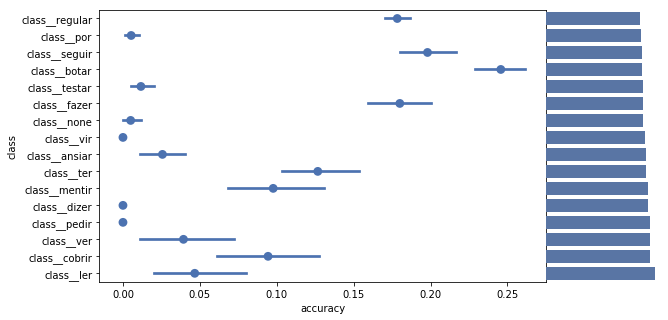
\includegraphics[width=0.8\linewidth]{img/accuracyperplexity.png}
  \caption{Acuracia por Perplexidade Ascendente}
  \label{fig:kfoldprop}
\end{figure}

Falar sobre o tamanho médio dos verbos alvo.

\begin{figure}[H]
  \centering
  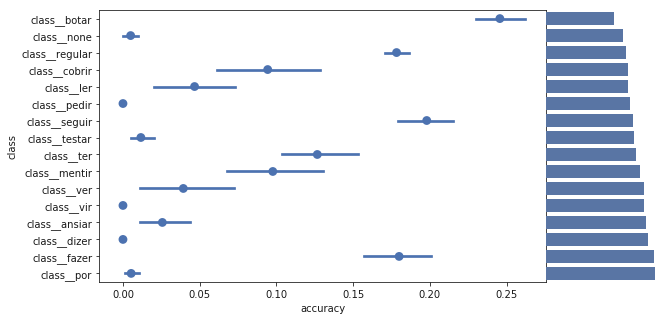
\includegraphics[width=1.0\linewidth]{img/accuracy_by_len.png}
  \caption{Acuracia por Cumprimento Medio Ascendente}
  \label{fig:kfoldprop}
\end{figure}


\section{Análise dos Erros}

Falar que eu escolhi o arquivo com a maior acuracia para analisar. Esse arquivo teve um total de 73 acertos, 17\% de acuracia.


\section{Arquivo com melhores resultados}

\begin{figure}[H]
  \centering
  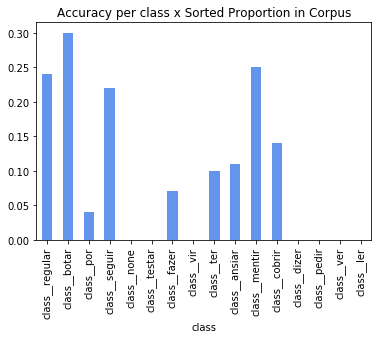
\includegraphics[width=0.7\linewidth]{img/best_file_accuracy.png}
  \caption{Acuracia proporcao corpus}
  \label{fig:acuraciaprop}
\end{figure}



\begin{figure}[H]
  \centering
  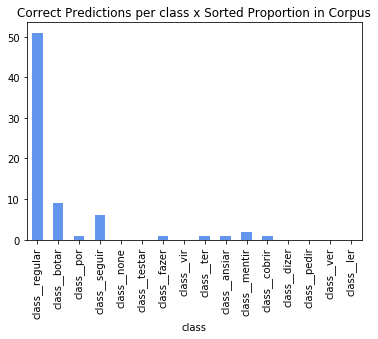
\includegraphics[width=0.7\linewidth]{img/best_file_correct_p.png}
  \caption{Predicoes corretas x proporcao}
  \label{fig:predicxprop}
\end{figure}

\begin{figure}[H]
  \centering
  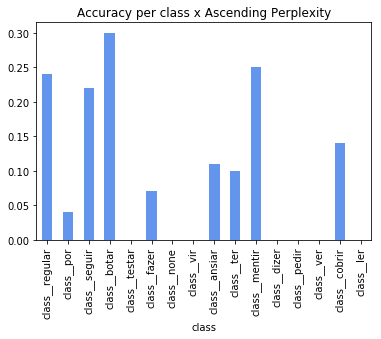
\includegraphics[width=0.7\linewidth]{img/best_file_acuracy_perplexity.png}
  \caption{acuracia perplexidade}
  \label{fig:acuper}
\end{figure}

\begin{figure}[H]
  \centering
  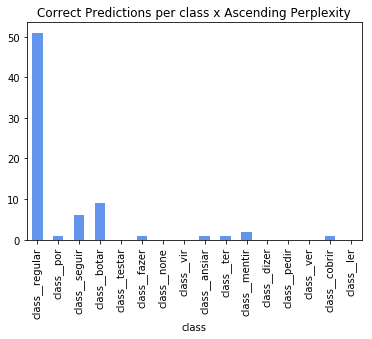
\includegraphics[width=0.7\linewidth]{img/best_file_accuracy_perplexity.png}
  \caption{prediçoes corretas x perplexidade}
  \label{fig:prexper}
\end{figure}


mostrar uma tabela com esse arquivo e analisar os erros encontrados

discussao dos resultados
cada classe
comentar sobre erros interessantes, por exemplo trocas de classes
experimentos com verbos inventados
